\documentclass{article}

\usepackage[%
    left=0.5in,%
    right=0.5in,%
    top=0.5in,%
    bottom=0.5in,%
]{geometry}%
\usepackage{minitoc}
\usepackage{multicol}
\usepackage{graphicx}
\usepackage{fixltx2e}
\usepackage{listings}
\usepackage{color}
\usepackage{hyperref}
    \hypersetup{ colorlinks = true, linkcolor = blue }
\usepackage{blindtext}
\definecolor{lightgray}{gray}{0.9}
\graphicspath{ {./} }

\definecolor{mygreen}{rgb}{0,0.6,0}
\definecolor{mygray}{rgb}{0.5,0.5,0.5}
\definecolor{mymauve}{rgb}{0.58,0,0.82}
 
%Customize a bit the look
\lstset{ %
backgroundcolor=\color{white}, % choose the background color; you must add \usepackage{color} or \usepackage{xcolor}
basicstyle=\footnotesize, % the size of the fonts that are used for the code
breakatwhitespace=false, % sets if automatic breaks should only happen at whitespace
breaklines=true, % sets automatic line breaking
captionpos=b, % sets the caption-position to bottom
commentstyle=\color{mygreen}, % comment style
deletekeywords={...}, % if you want to delete keywords from the given language
escapeinside={\%*}{*)}, % if you want to add LaTeX within your code
extendedchars=true, % lets you use non-ASCII characters; for 8-bits encodings only, does not work with UTF-8
frame=single, % adds a frame around the code
keepspaces=true, % keeps spaces in text, useful for keeping indentation of code (possibly needs columns=flexible)
keywordstyle=\color{blue}, % keyword style
% language=Octave, % the language of the code
morekeywords={*,...}, % if you want to add more keywords to the set
numbers=left, % where to put the line-numbers; possible values are (none, left, right)
numbersep=5pt, % how far the line-numbers are from the code
numberstyle=\tiny\color{mygray}, % the style that is used for the line-numbers
rulecolor=\color{black}, % if not set, the frame-color may be changed on line-breaks within not-black text (e.g. comments (green here))
showspaces=false, % show spaces everywhere adding particular underscores; it overrides 'showstringspaces'
showstringspaces=false, % underline spaces within strings only
showtabs=false, % show tabs within strings adding particular underscores
stepnumber=1, % the step between two line-numbers. If it's 1, each line will be numbered
stringstyle=\color{mymauve}, % string literal style
tabsize=2, % sets default tabsize to 2 spaces
title=\lstname % show the filename of files included with \lstinputlisting; also try caption instead of title
}
%END of listing package%
 
\definecolor{darkgray}{rgb}{.4,.4,.4}
\definecolor{purple}{rgb}{0.65, 0.12, 0.82}
 
%define Javascript language
\lstdefinelanguage{JavaScript}{
keywords={typeof, new, true, false, catch, function, return, null, catch, switch, var, if, in, while, do, else, case, break, const},
keywordstyle=\color{blue}\bfseries,
ndkeywords={class, export, boolean, throw, implements, import, this},
ndkeywordstyle=\color{darkgray}\bfseries,
identifierstyle=\color{black},
sensitive=false,
comment=[l]{//},
morecomment=[s]{/*}{*/},
commentstyle=\color{purple}\ttfamily,
stringstyle=\color{red}\ttfamily,
morestring=[b]',
morestring=[b]"
}
 
\lstset{
language=JavaScript,
extendedchars=true,
basicstyle=\footnotesize\ttfamily,
showstringspaces=false,
showspaces=false,
numbers=left,
numberstyle=\footnotesize,
numbersep=9pt,
tabsize=2,
breaklines=true,
showtabs=false,
captionpos=b
}

\newcommand{\inlinecode}[2]{\colorbox{lightgray}{\lstinline
[language=#1]$#2$}}
\newcommand{\worddef}[1]{\hyperref[sec:reference]{\textit{#1}}}

\usepackage{blindtext}
\title{G53DEV Final report}
\author{Augustinas Jokubauskas (psyaj1)}

\begin{document}

\maketitle

\begin{flushleft}
When looking at github commits, some might say username of Knightls or Augustinas, that happened because I had configured github incorrectly. All the charts are taken from and can be confirmed on \href{https://npm-stat.com}{npm-stat}
\end{flushleft}

\pagebreak

\tableofcontents

\newpage

\section{Dlister}

\subsection{About}

\begin{flushleft}
\texttt{dlister} was created on \textbf{05/02/2017} and can be found on \href{https://github.com/WhoAteDaCake/dlister}{Github}. \\
It's a cli tool, which allows to quickly and easily list directory trees and files within them. It's build on top of node.js which allows it to be used as a universal tool with extremely simple installation on a large number of operating systems. Dlister also has a stackoverflow integration allowing for painless project layout display when creating a question. I am currently the sole maintainer of the project, which lead to development being slowed down recently, however there are plans for a complete rewrite in ocaml using bucklescript compiler to transform it to javascript. This would mean being able to utilise ocaml's type system to produce better quality code.
\end{flushleft}

\subsection{Example usage}

\begin{multicols}{2}
  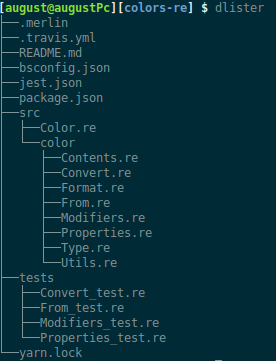
\includegraphics[scale=0.5]{dlister_use.png}
  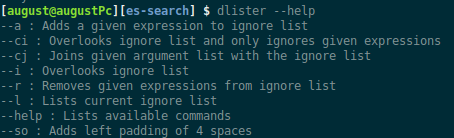
\includegraphics[scale=0.8]{dlister_help.png}
\end{multicols}

\pagebreak

\subsection{Statistics}
\begin{flushleft}
Between 05/02/2017 and 26/09/2018 package has been downloaded \textbf{2297} times
\end{flushleft}

\begin{center}
  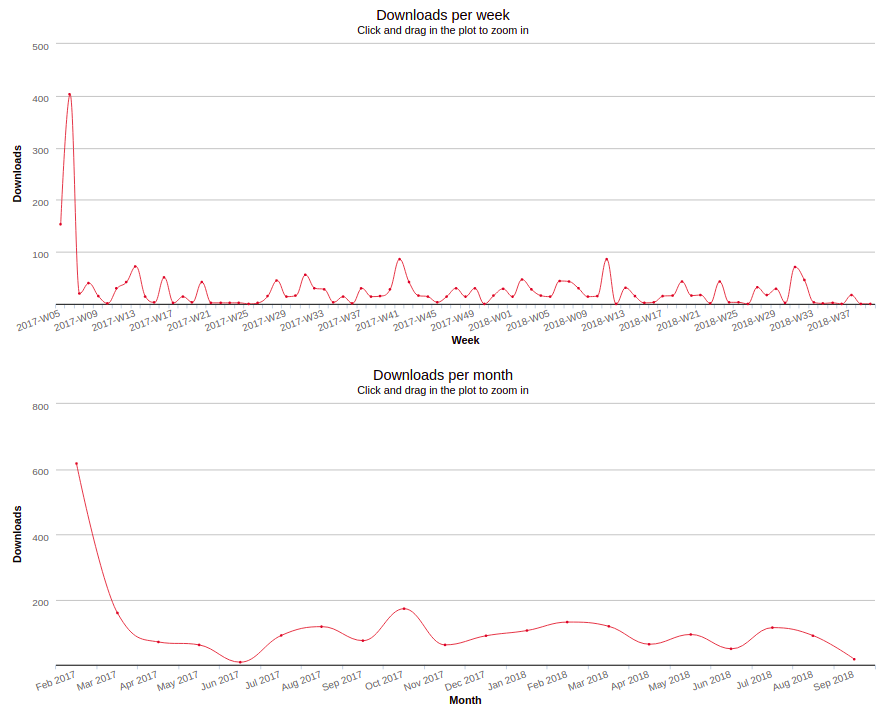
\includegraphics[scale=0.5]{dlister.png}
\end{center}

\newpage

\section{react-routes-map}

\subsection{About}
\begin{flushleft}
\texttt{react-routes-map} was created on \textbf{27/09/2017} and can be found on \href{https://github.com/WhoAteDaCake/react-router-map}{Github}.\\
This tool was made to simply react developers lives by dynamically generating routes for a single page application. react-routes-map saves hundreds of lines of codes as well as making configuration as simple as just a single JSON object, while it also allows users to customise route imports as well as setting custom loading actions. Using dynamic importing of routes also has an added benefit of drastically reducing bundle sizes, which in return will speed up initial page load times. I am currently the sole maintainer of the project, however, due to the nature of the project, it does not require often maintenance.
\end{flushleft}

\subsection{Example usage}

\begin{lstlisting}[language=Javascript]
import mapRoutes from 'react-routes-map';
 
const routes = [
  {
    path: '/home',
    component: 'Home',
    name: 'Home'
  }, {
    path: '/projects',
    component: 'Projects',
    name: 'Projects',
    children: [
      {
        path: '/add',
        component: 'ProjectForm',
      },
    ],
  }, {
    path: false,
    component: 'Default',
  }
];
 
const options = {
  Loading: props => <span>loading...</span>,
  loader() {
    return import(`./${component}`)
      .catch(e => import(`./${component}/index.js`));
  }
}
 
export default mapRoutes(routes, options);
\end{lstlisting}

\pagebreak

\subsection{Statistics}
\begin{flushleft}
Between 27/09/2017 and 26/09/2018 package has been downloaded \textbf{1283} times
\end{flushleft}

\begin{center}
  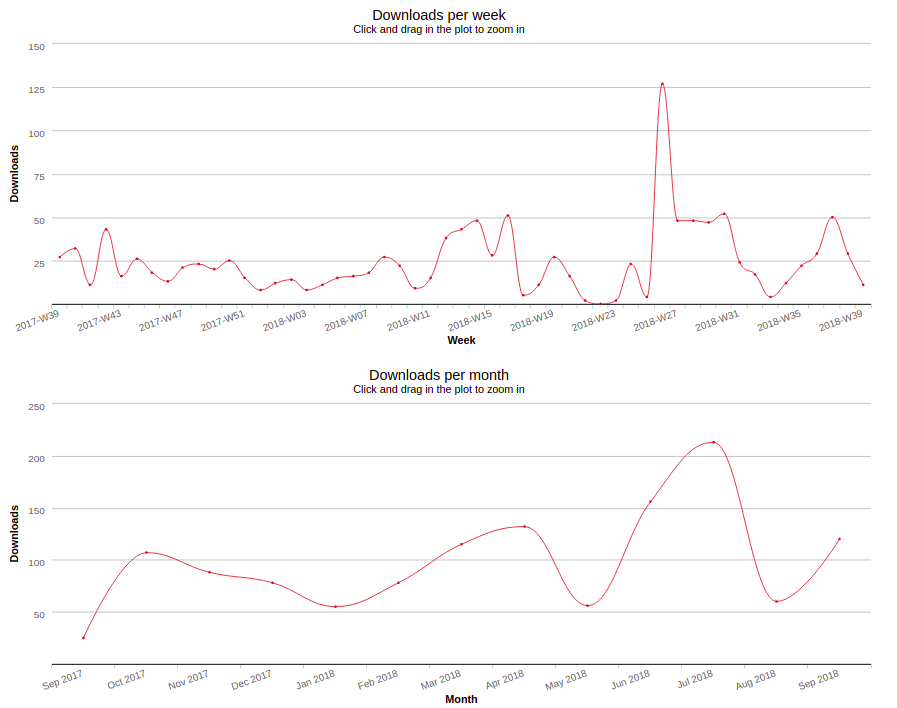
\includegraphics[scale=0.5]{react-routes-map.png}
\end{center}

\newpage

\section{color-re}

\subsection{About}
\begin{flushleft}
\texttt{color-re} packages was created on \textbf{19/06/2018} and can be found \href{https://github.com/WhoAteDaCake/color-re}{Github} \\
This package is a rework of \href{https://github.com/Qix-/color}{color} package in reason. It has 0 dependencies as well as only being \texttt{120K} in size. Due to the package being written in reason, it's strongly typed, which prevents common runtime errors which are horrible to debug. It can be easily integrated with reason, javascript and ocaml projects, this allows for an easier code reuse between projects. I am currently the sole maintainer of the project. color-re package currently provides all core functionality required, so there is no need for maintenance.
\end{flushleft}

\subsection{Example usage}

\begin{lstlisting}
/* Change the opacity */
Color.(fromRgb((200, 200, 200)) |> opacity(1.5) |> toString) |> Js.log
Color.(fromRgb((200, 200, 200)) |> toHsl |> fade(0.5) |> toString) |> Js.log
Color.(fromRgb((200, 200, 200)) |> toHsl |> opaquer(0.4) |> toString) |> Js.log

/* Color convertions */
Color.(fromRgb((200, 200, 200)) |> toHex |> toHsl |> toHsv |> toString) |> Js.log

/* Color properties */
Color.(fromRgb((200, 200, 200)) |> luminosity) |> Belt.Option.getExn |> Js.log
Color.(fromRgb((200, 200, 200)) |> contrast(fromHex("#aaafff"))) |> Belt.Option.getExn |> Js.log
\end{lstlisting}

\subsection{Statistics}
\begin{flushleft}
Between 19/06/2018 and 26/09/2018 package has been downloaded \textbf{227} times
\end{flushleft}

\begin{center}
  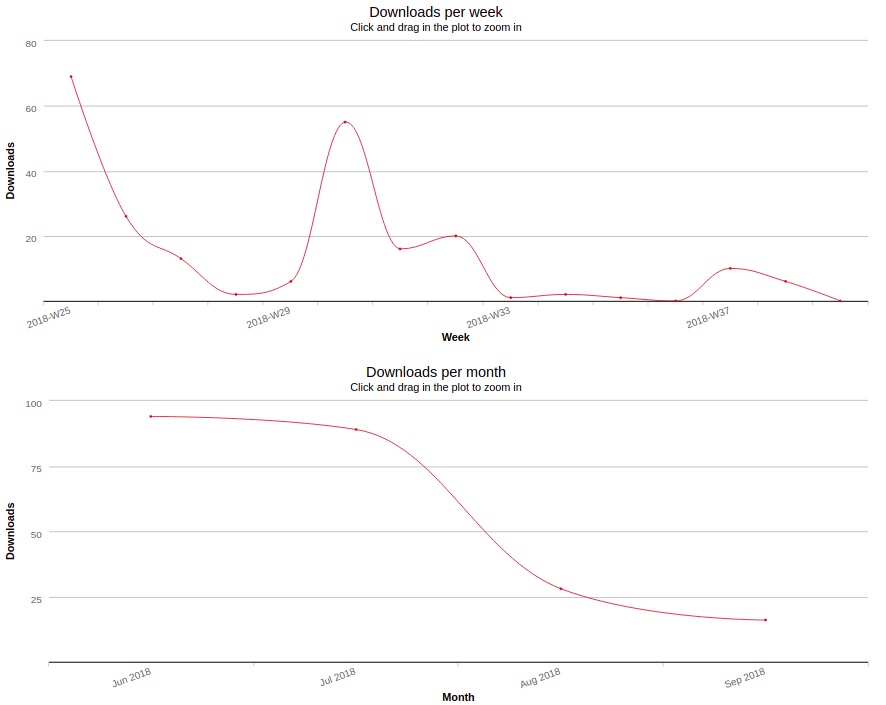
\includegraphics[scale=0.5]{color-re.png}
\end{center}

\newpage

\section{@atecake/builder}

\subsection{About}

\begin{flushleft}
\texttt{@atecake/builder} was created on \textbf{11/09/2018} and can be found on \href{https://github.com/WhoAteDaCake/builder}{Github} \\
This package that helps to publish/develop javascript libraries. It simplifies build dependencies as well as makes it extremelly easy to tag releases. While it allows starting with very simple configuration, it also allows for customisation. It has built in support for multiple file types used in web-development, which helps to cut down in number of dependencies. I am currently a sole maintainer of this project. It's still in an alpha stage and I plan to add better documentation as well as improving the performance and usability.
\end{flushleft}

\subsection{Example usage}
\begin{lstlisting}[language=Javascript]
const {
  start,
  devServer,
  when,
  bundle,
  library,
  configure,
  customise,
  tag,
  tap,
} = require('@atecake/builder');

const pkg = require('./package.json');

start([
  configure(),
  when('build', [
    bundle({ files: { input: 'src/index.js', output: pkg.main } }),
    bundle({
      files: { input: 'src/index.js', output: pkg.module },
      build: { rollup: { format: 'esm' } },
      action: Promise.resolve(),
    }),
    library({
      files: { input: 'src', output: 'lib' },
      build: { rollup: { format: 'cjs' } },
      action: Promise.resolve(),
    }),
  ]),
  when('start', [devServer()]),
  when('tag', [tag()]),
]);
\end{lstlisting}

\pagebreak

\subsection{Statistics}
\begin{flushleft}
Between 11/09/2018 and 26/09/2018 package has been downloaded \textbf{259} times
\end{flushleft}

\begin{center}
  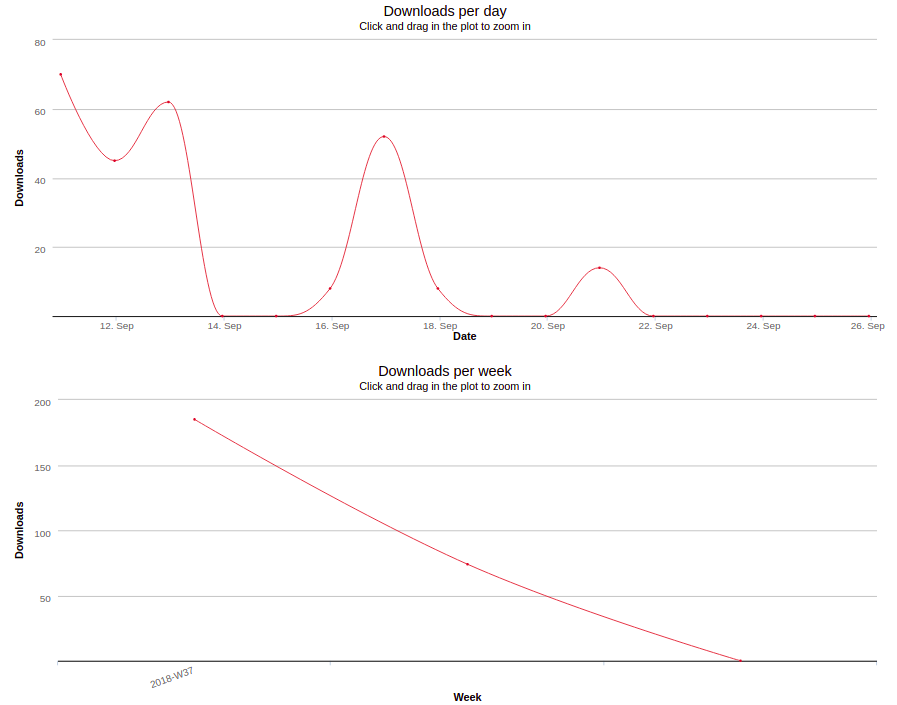
\includegraphics[scale=0.5]{builder.png}
\end{center}

\newpage

\section{@spotlightdata/nanowire-extensions}

\subsection{About}
\begin{flushleft}
\texttt{@spotlightdata/nanowire-extensions} was created on \textbf{19/06/2018} and can be found on \href{https://github.com/SpotlightData/nanowire-extensions}{Github}\\
This is common component package built on top of \href{https://ant.design/docs/react/introduce}{ant design}. Due to the way the components and helper functions are structed, the library can be re-used accross different platforms. The component seperation has allowed each part to be documented as well tested, so that the developers only need to worry about the integration of components.
\end{flushleft}

\subsection{Example usage}

\begin{center}
  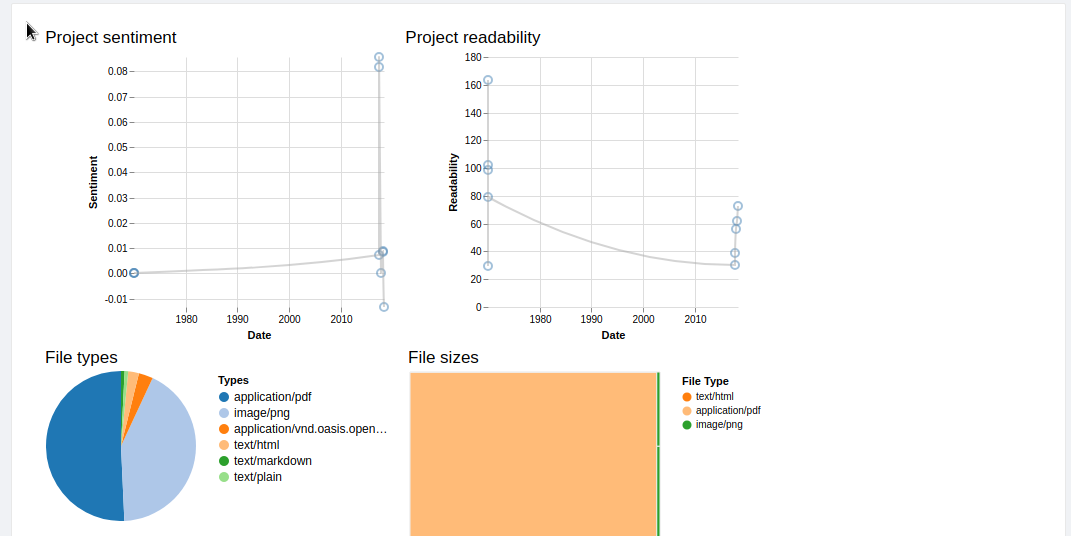
\includegraphics[scale=0.5]{Screenshot_2018-09-28_11-44-09.png}
\end{center}

\pagebreak

\subsection{Statistics}

\begin{flushleft}
Between 19/06/2018 and 26/09/2018 package has been downloaded \textbf{3430} times
\end{flushleft}

\begin{center}
  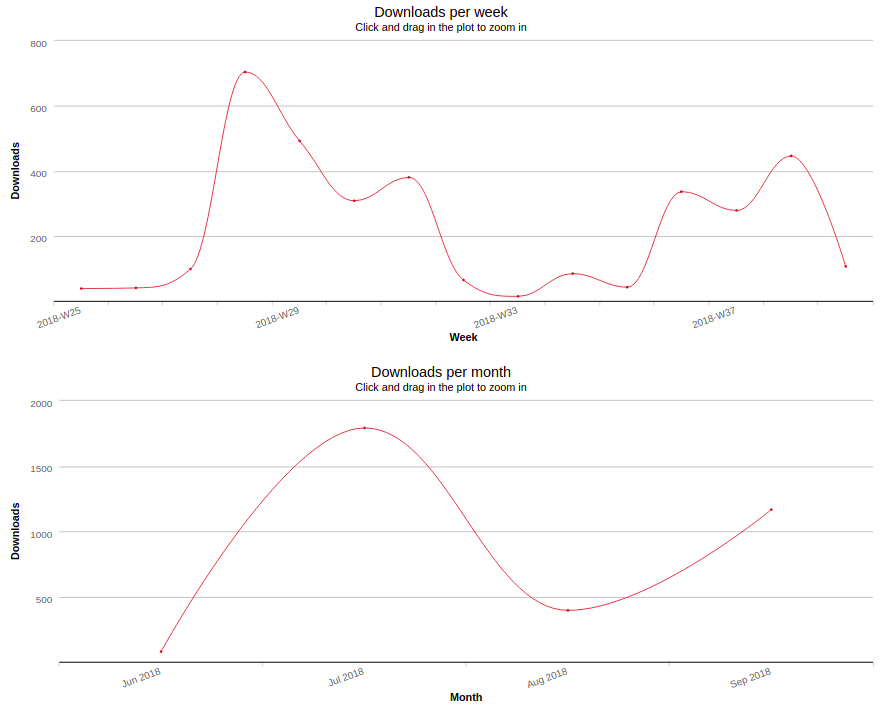
\includegraphics[scale=0.5]{extensions.png}
\end{center}

\newpage

\section{@spotlightdata/es-search}

\subsection{About}
\begin{flushleft}
This project was created on \textbf{06/09/2018} and can be found on \href{https://github.com/SpotlightData/es-search}{Github} \\
This package is a wrapper for comonly used searchkit components, It simplifies the usage of as well as fixes common searchkit library issues.
\end{flushleft}

\subsection{Example usage}

\begin{center}
  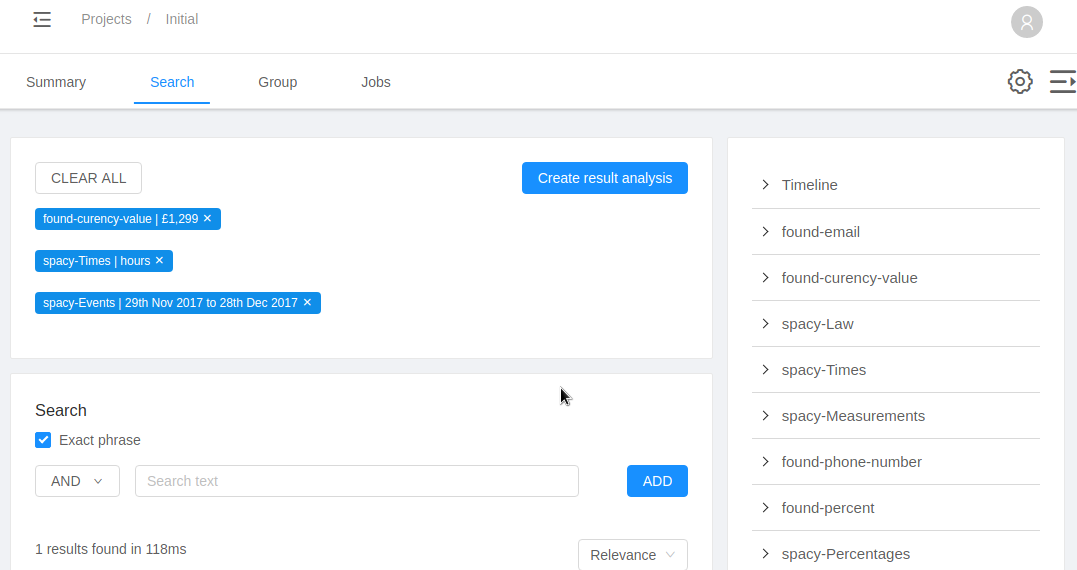
\includegraphics[scale=0.5]{Screenshot_2018-09-28_11-43-45.png}
\end{center}

\pagebreak

\subsection{Statistics}

\begin{flushleft}
Between 06/09/2018 and 26/09/2018 package has been downloaded \textbf{972} times
\end{flushleft}

\begin{center}
  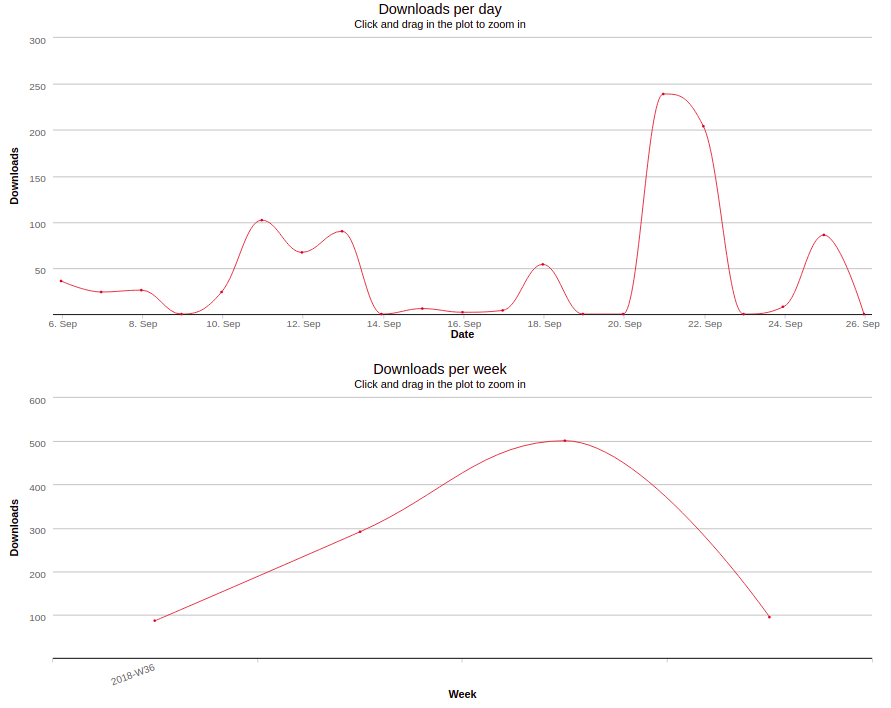
\includegraphics[scale=0.5]{es-search.png}
\end{center}

\newpage

\section{@spotlightdata/document-viewer}

\subsection{About}
\begin{flushleft}
This package was created on \textbf{22/08/2018} and can be found on \href{https://github.com/SpotlightData/react-lazylog}{Github}\\
This package is a fork of \href{https://github.com/mozilla-frontend-infra/react-lazylog}{react-lazylog}. It uses fundamentals of the forked project, however it's purpose is vastly different. It has been made to allow large files (< 30mb in size) to be readable and dynamically loaded in the browser. It also features a fully functional text and positional entity search.
\end{flushleft}

\subsection{Example usage}

\begin{center}
  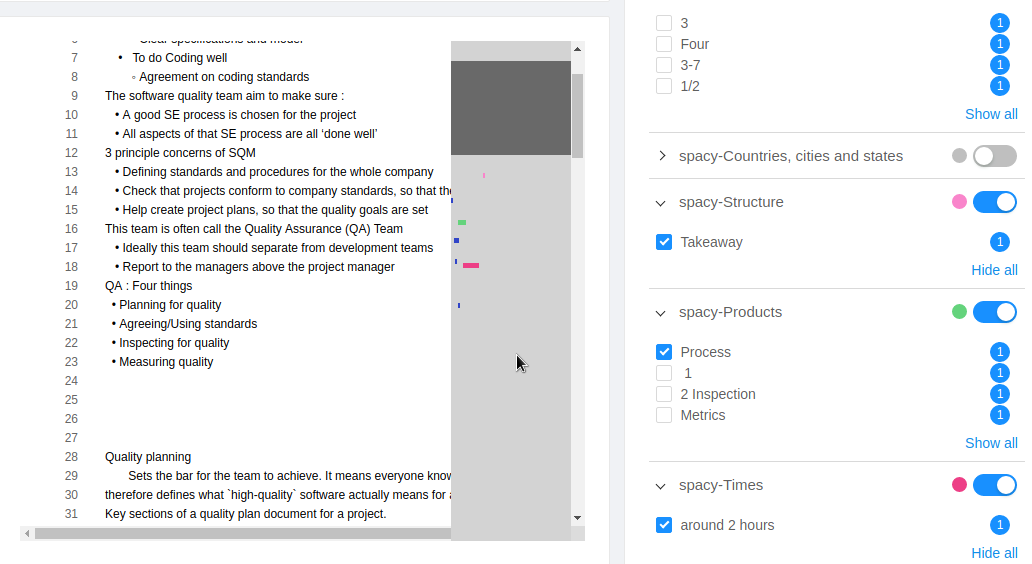
\includegraphics[scale=0.5]{Screenshot_2018-09-28_11-42-57.png}
\end{center}

\pagebreak

\subsection{Statistics}

\begin{flushleft}
Between 22/08/2018 and 26/09/2018 package has been downloaded \textbf{754} times
\end{flushleft}

\begin{center}
  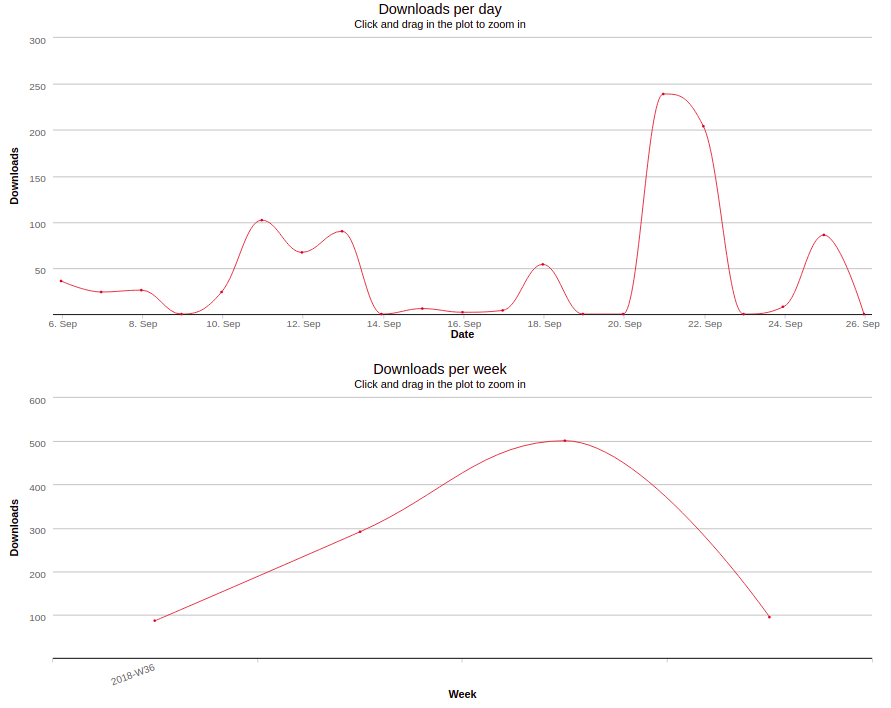
\includegraphics[scale=0.5]{es-search.png}
\end{center}



\end{document}
